\documentclass{article}

\usepackage[preprint,nonatbib]{neurips_2026}
\makeatletter
\renewcommand{\@notice}{\enlargethispage{2\baselineskip}}
\makeatother
\raggedbottom

\usepackage[utf8]{inputenc}
\usepackage[T1]{fontenc}
\usepackage{graphicx}
\usepackage{amsmath}
\usepackage{amssymb}
\usepackage{booktabs}
\usepackage{xcolor}
\usepackage{hyperref}
\usepackage{microtype}
\usepackage{caption}
\usepackage{float}
\usepackage[numbers,sort&compress]{natbib}
\renewcommand{\arraystretch}{0.92}
\setlength{\tabcolsep}{3.5pt}
\captionsetup{skip=5pt}
\setlength{\textfloatsep}{3pt plus 1pt minus 1pt}
\setlength{\intextsep}{2pt plus 1pt minus 1pt}
\setlength{\abovedisplayskip}{2pt plus 1pt minus 1pt}
\setlength{\belowdisplayskip}{2pt plus 1pt minus 1pt}
\setlength{\parskip}{0pt}
\setlength{\abovecaptionskip}{5pt}
\setlength{\belowcaptionskip}{2pt}

\newcommand{\tbd}[1]{\textcolor{red}{#1}}

\title{What Post-Training Optimizes: Controlled Studies of Preference, Group, and Verifiable Feedback in a Small Language Model}

\author{
  Mohid Ali \\
  Lahore University of Management Sciences (LUMS) \\
  \texttt{28100043@lums.edu.pk}
}

\begin{document}

\maketitle

\begin{abstract}
A post-trained model is only as dependable as the objective and the feedback
that shaped it. This report tests that claim with five controlled experiments on
one small instruction tuned model. It starts from the most basic signal, fixed
preference pairs, and studies how an offline objective changes with its
regularization strength and with the length balance of its data. It then moves
to online training, where the model generates its own samples under a critic,
and to a variant that drops the critic and ranks samples within a group. Every
method is tested along its main control. Next, the trained policies are checked
for needless refusal and harmful compliance by an AI judge whose agreement with
manual labels is measured. The final experiment holds the optimizer constant and
varies the source of feedback, setting an exact answer checker against an AI
judge on perturbed versions of correct responses. Across the experiments, the
measurements behind a score explain behavior better than the score itself. They
reveal a preference margin that depends on length, a critic with negative
explained variance, a judge that cannot tell a justified refusal from a needless
one, and a judge that depends on style. Code, configurations, and full result tables are
available at \url{https://github.com/Mohidali2005/ATML_PA2}.
\end{abstract}

\section{Introduction}
\label{sec:intro}

How much a post-trained language model can be trusted depends on the objective
and the feedback that guided its training. Every training signal is a proxy for
the behavior a user wants. A preference likelihood, a learned reward, and an
answer checker each capture part of that behavior and miss the rest. The
training curves give no warning when the proxy and the intended behavior start
to differ. This report follows that gap from the simplest training signal to the question of
where the signal should come from.

The simplest signal is a fixed set of preference pairs. Direct Preference
Optimization (DPO) \citep{rafailov2023direct} learns from such pairs against a
frozen reference policy, with no reward model and no sampling. Fixed data carries
biases of its own, and response length is a known one
\citep{singhal2023long,park2024disentangling}. The first study therefore varies
the regularization strength and the length balance of the pairs. DPO never sees
its own outputs, which raises the next question of what changes when the policy
generates the data it learns from.

Online methods answer that by sampling responses and scoring them with a reward
model. Proximal Policy Optimization (PPO)
\citep{schulman2017proximal} adds a learned critic with two separate controls, a
clipping range and a reference penalty, and a learned reward reduces as the
policy diverges from its starting point \citep{gao2023scaling}. Group Relative
Policy Optimization (GRPO) \citep{shao2024deepseekmath} removes the critic, a
component that can fail, and compares several samples of one prompt. This moves
the burden onto reward variation inside each group and onto how long and short
completions are weighted \citep{liu2025understanding}. The second and third
studies test each method along these controls.

A higher reward does not guarantee better behavior, whichever method is used. A
model can lower harmful compliance simply by refusing more
\citep{bianchi2024safetytuned}, which an exaggerated safety benchmark such as
XSTest \citep{rottger2024xstest} is built to expose. The fourth study therefore
checks the trained policies for needless refusal and harmful compliance with an
AI judge, whose agreement with manual labels is measured. This raises the last
question of where feedback should come from. An exact verifier gives a
reproducible but sparse signal \citep{deepseekai2025r1}, while an AI judge gives
a graded signal with its own biases and cost
\citep{lee2024rlaif,bai2022constitutional,zheng2023judging}. The fifth study
changes only the source of feedback. Together, the five studies ask how much a
model can be trusted when its objective and feedback are imperfect proxies, and
which measurements show when they are not.

\section{Shared Experimental Setup}
\label{sec:setup}

Every study uses Qwen2.5-1.5B-Instruct \citep{qwen2024qwen25} as the base model,
with trainable low rank adapters \citep{hu2022lora} on the attention query and
value projections. DPO starts from the instruction tuned model and trains on
UltraFeedback preference pairs \citep{cui2024ultrafeedback}. PPO and GRPO
continue from supplied midpoint adapters. Both draw prompts from one shared
UltraFeedback pool and score responses with one fixed reward model. PPO also
starts from a supplied value model. Within a study, every comparison keeps the
same prompts, decoding settings, seed, and starting checkpoint. The evaluation
sets are small, so each paired per prompt difference is reported with its
standard error. A difference below about two standard errors is not read as an
effect. Reward scores are compared only within one task.

\section{Task 1: Direct Preference Optimization}
\label{sec:task1}

\subsection{Methodology}

DPO fits the policy on pairs of a preferred response $y^{+}$ and a rejected
response $y^{-}$ with the loss:
\begin{equation}
\begin{aligned}
  \mathcal{L}_{\text{DPO}} &= -\,\mathbb{E}\big[\log\sigma(\beta\, m)\big],\\
  m &= \big[\ell_\theta(y^{+})-\ell_\theta(y^{-})\big]-\big[\ell_{\text{ref}}(y^{+})-\ell_{\text{ref}}(y^{-})\big],
\end{aligned}
  \label{eq:dpo}
\end{equation}
where $\ell(y)=\log\pi(y\mid x)$ is the sequence log probability, summed over
response tokens, and the reference is the same policy with the adapter
switched off \citep{rafailov2023direct}. The quantity $m$ is the margin, and
preference accuracy is the share of held out pairs with a positive margin, so
it measures movement relative to the reference. Prompts are always kept whole and
responses are truncated from the right, so pairs whose prompt alone reaches the
768 token limit are dropped, leaving 1446 training pairs and 290 held out pairs. The standard run trains for one epoch at $\beta=0.1$. The
regularization study trains forks for $\beta\in\{0.03,0.1,0.3\}$ on a shorter
run of 600 pairs. The length study trains a second model on a supplied set
with equal counts of pairs where the preferred response is longer, matched in
length, or shorter. Both models are evaluated on a stratified held out set of
237 pairs and on ten prompts that state a word limit.

\subsection{Results}

\begin{table}[!htb]
  \centering
  \small
  \begin{tabular}{lccccc}
    \toprule
    Condition & DPO loss & Pref. acc. & Sampled KL & Reward ($\pm$SE) & Length (std) \\
    \midrule
    Standard, full epoch ($\beta=0.1$) & 0.674 & 0.497 & $3.3\times10^{-4}$ & 1.378 $\pm$ 0.067 & 156.0 (104.7) \\
    Short fork, $\beta=0.03$           & 0.691 & 0.500 & $2.7\times10^{-5}$ & 1.303 $\pm$ 0.068 & 153.1 (106.1) \\
    Short fork, $\beta=0.1$            & 0.687 & 0.493 & $-1.7\times10^{-5}$ & 1.259 $\pm$ 0.070 & 152.8 (105.4) \\
    Short fork, $\beta=0.3$            & 0.678 & 0.493 & $-1.5\times10^{-4}$ & 1.389 $\pm$ 0.068 & 153.5 (104.9) \\
    \bottomrule
  \end{tabular}
  \vspace{8pt}
  \caption{Held out results on 290 pairs. The standard run and the short forks
  use different training sizes (1446 versus 600 pairs), so only the forks are directly
  comparable. The standard error of preference accuracy is 0.029.}
  \label{tab:task1-main}
\end{table}

Training loss falls from 0.694 over the first ten steps to 0.669 over the last
ten (Appendix Figure~\ref{fig:app-dpo}), and the held out loss is 0.674 (Table~\ref{tab:task1-main}). Held out
preference accuracy is 0.497 and sampled KL is $3.3\times10^{-4}$. A margin this
close to zero is dominated by noise, so its sign says little about which response
was preferred. A rank 8 adapter at a learning rate of $2\times10^{-5}$ for 91
steps has barely moved the policy from the reference, which explains all three
numbers. The $\beta$ study
shows no consistent trend (Appendix Figure~\ref{fig:app-beta}), since each short
fork leaves the margin too close to zero for $\beta$ to act on. Accuracy is 0.500, 0.493, and 0.493, KL stays
within a few $10^{-4}$ of zero with a changing sign, and reward is 1.303, 1.259,
and 1.389, all within about two standard errors of each other. Only the held out
loss falls steadily as $\beta$ grows, and that is a scale effect. For margins near zero the
loss is approximately $\ln 2-\beta\bar m/2$, so a larger $\beta$ lowers it by
scaling a similar mean margin of roughly 0.1 to 0.15 nats.

\begin{table}[!htb]
  \centering
  \footnotesize
  \begin{tabular}{lccccc}
    \toprule
    Policy & Pref. longer (78) & Matched (80) & Rej. longer (79) & Word limit tokens & Compliance \\
    \midrule
    Standard        & 0.462 & 0.600 & 0.658 & 45.5 & 6 of 10 \\
    Length balanced & 0.449 & 0.600 & 0.785 & 46.4 & 6 of 10 \\
    \bottomrule
  \end{tabular}
  \vspace{8pt}
  \caption{Held out preference accuracy by length stratum on 237 pairs, with
  the stratum sizes in brackets, and generated length and word limit
  compliance on ten prompts.}
  \label{tab:task1-length}
\end{table}

The stratified evaluation shows what the margin tracks (Table~\ref{tab:task1-length}).
The standard policy scores 0.46 when the preferred response is longer
and 0.66 when the rejected response is longer. The gap of 0.20 between them is
about 2.5 standard errors. Sequence log probabilities sum over tokens, so a small
shift away from the reference accumulates over more tokens in a longer response,
and the margin follows which response is shorter. That direction is the opposite
of the verbosity bias reported for DPO
\citep{singhal2023long,park2024disentangling}. A plausible reason is that one
short epoch has not yet taught the policy the preference for longer responses
those studies describe. The two models generate responses
of the same length, so on this short run the length dependence is a property of
the margin. Training on the balanced pairs does not remove it. Accuracy stays at
0.45 for preferred longer pairs and rises to 0.78 for rejected longer pairs. It
might be because balancing removes the length pattern of the standard
pairs and leaves the token count effect as the main influence on the margin.
Overall stratified accuracy is
0.574 against 0.612, which is 9 pairs out of 237 and inside noise.

Reward and quality separate in two ways. A question that asks only to name one
famous person from Calcutta with a Nobel Prize scored 3.21, among the highest
rewards on the held out set. The response names Amartya Sen correctly and then
adds an invented ``St.\ Martin's College'' and a Templeton Prize that Sen did
not receive. The word limit prompts show the same gap for instruction following. The
standard model wrote 93 words against a limit of 45 on one prompt, and the
balanced model wrote 72 words against a limit of 35 on another. A stronger
preference signal can therefore coexist with worse correctness and concision,
because the training pairs never test a stated limit.

\section{Task 2: Proximal Policy Optimization}
\label{sec:task2}

\subsection{Methodology}

In Task~1 the policy used a fixed dataset, whereas PPO generates the responses it
learns from. It continues the supplied midpoint for 20 updates, each on one
prompt with two optimization epochs over 512 token rollouts. The policy maximizes the
clipped surrogate:
\begin{equation}
  \mathcal{L}_{\text{clip}} = \mathbb{E}_t\big[\min\big(\rho_t A_t,\ \mathrm{clip}(\rho_t,1-\epsilon,1+\epsilon)A_t\big)\big],\qquad \rho_t=\frac{\pi_\theta(a_t\mid s_t)}{\pi_{\text{old}}(a_t\mid s_t)},
  \label{eq:ppo}
\end{equation}
where $A_t$ comes from generalized advantage estimation
\citep{schulman2016high} over a learned value model and a token reward
$r_t=r_{\text{task}}\mathbf{1}[t=T]-\beta_{\text{KL}}(\log\pi_\theta-\log\pi_{\text{ref}})$.
The range $\epsilon$ limits how far one batch can move a token probability,
and $\beta_{\text{KL}}$ punishes distance from the reference over many updates.
The clipping study counts
tokens with a ratio outside $[1-\epsilon,1+\epsilon]$ on a cached batch of 32
rollouts over ten optimizer steps and in a drift stress test that takes the
ratio between the rollout policy and the reference. It also trains eight
update forks for $\epsilon\in\{0.05,0.2,0.5\}$. The KL study trains forks for
$\beta_{\text{KL}}\in\{0,0.1,0.2\}$ at $\epsilon=0.2$. Stability is the mean absolute ratio deviation after each update and the peak gradient norm.

\subsection{Results}

\begin{table}[!htb]
  \centering
  \small
  \begin{tabular}{lcc}
    \toprule
    Quantity over 20 updates & PPO & GRPO \\
    \midrule
    Reward, mean [min, max]            & 1.62 [$-2.45$, 3.42] & 1.53 [$-0.20$, 3.00] \\
    Sampled KL, mean [min, max]        & $1\times10^{-5}$ [$-6\times10^{-4}$, $6\times10^{-4}$] & $6\times10^{-5}$ [$-3\times10^{-4}$, $4\times10^{-4}$] \\
    Entropy, mean [min, max]           & 0.89 [0.41, 2.16] & 0.83 [0.21, 1.65] \\
    Response length, mean [min, max]   & 301 [70, 512] & 278 [54, 512] \\
    Policy loss / value loss, mean     & $-3\times10^{-5}$ / 3.11 & $-0.028$ / -- \\
    Clip fraction                      & 0.000 & 0.000 \\
    Gradient norm, mean (peak)         & 0.34 (0.81) & 0.26 (0.97) \\
    Group reward std / uninformative   & -- & 0.73 / 0.000 \\
    Wall clock, peak memory            & 329 s, 9.6 GB & 448 s, 9.9 GB \\
    \bottomrule
  \end{tabular}
  \vspace{8pt}
  \caption{Standard continuation diagnostics for Tasks~2 and~3. Each update
  uses one prompt, so the ranges reflect prompt to prompt variation.
  Per update trajectories are in Appendix Figures~\ref{fig:app-ppo} and
  \ref{fig:app-grpo}.}
  \label{tab:trajectories}
\end{table}

\begin{figure}[!htb]
  \centering
  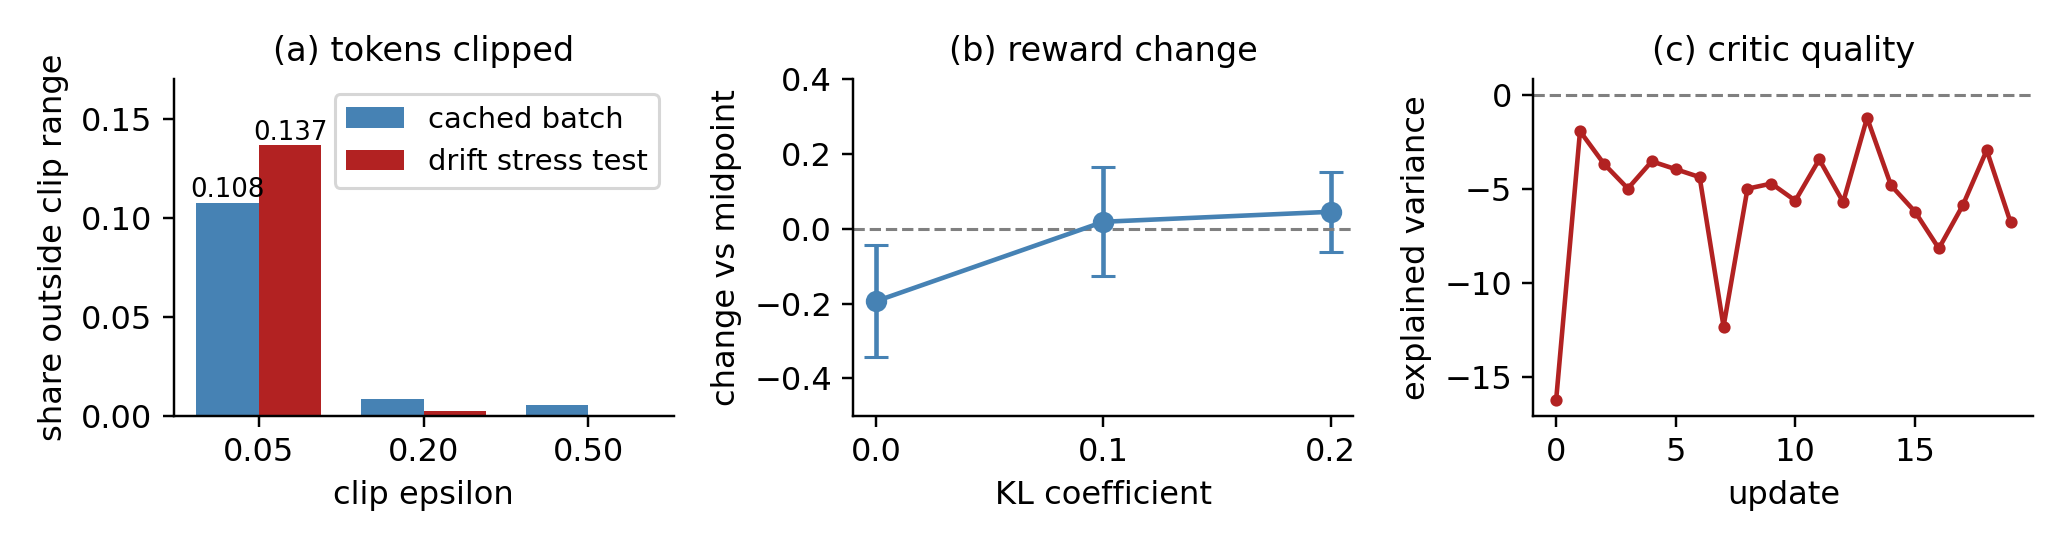
\includegraphics[width=\linewidth]{figures/task2_ppo_summary.png}
  \caption{\textbf{Clipping binds only when the ratio is measured away from
  the live policy, and the critic is worse than a constant.} (a) Tokens
  outside the clip range for each $\epsilon$ on the cached batch and in the
  drift stress test. (b) Paired held out reward change against the midpoint
  for each KL coefficient, with one standard error. (c) Critic explained
  variance over the 20 standard updates.}
  \label{fig:task2}
\end{figure}

Reward per update shows no trend (Table~\ref{tab:trajectories}). Held out reward moves
from 1.572 at the midpoint to 1.589, with a paired change of $+0.018\pm0.136$.
Entropy, length, and KL stay the same. The critic is the clearest problem. Its
explained variance averages $-5.6$ (Figure~\ref{fig:task2}c), so predicting the
mean return would beat it, and advantages built on it say little about which
tokens helped.

Clipping never binds in the live runs. The ratio deviation after an update is
at most 0.0045, more than ten times inside the tightest range of 0.05, so the
three $\epsilon$ forks follow one path and agree on every reported number
(Table~\ref{tab:task2}). The cached batch looks different
(Figure~\ref{fig:task2}a). The share of affected tokens falls from 10.8\% at
$\epsilon=0.05$ to 0.9\% and 0.6\%. The ratio deviation there is already 0.036
at step zero and stays flat over ten steps. That deviation is a numerical gap
between stored log probabilities and a fresh forward pass, so part of the clip
fraction is noise. The drift stress test has no such gap. It affects 13.7\% of
tokens at 0.05, 0.26\% at 0.2, and none at 0.5, although the mean ratio
deviation is only 0.0185. The difference between the rollout policy and the
reference is large only because of a small share of tokens.

\begin{table}[!htb]
  \centering
  \small
  \begin{tabular}{lcccccc}
    \toprule
    Condition & Reward $\Delta$ ($\pm$SE) & KL & Entropy & Length & Peak grad. & Critic EV \\
    \midrule
    Midpoint (start)                              & 1.572 & $-1.1\times10^{-5}$ & 0.807 & 291.5 & -- & -- \\
    $\epsilon$ sweep, $\beta_{\text{KL}}=0.1$ & $+0.019\pm0.146$ & $-3.8\times10^{-5}$ & 0.793 & 304.6 & 0.81 & $-6.4$ \\
    $\beta_{\text{KL}}=0$                         & $-0.193\pm0.150$ & $-4.3\times10^{-5}$ & 0.820 & 297.3 & 1.38 & $-12.4$ \\
    $\beta_{\text{KL}}=0.2$                       & $+0.046\pm0.107$ & $+2.2\times10^{-6}$ & 0.779 & 298.8 & 0.80 & $-6.4$ \\
    \bottomrule
  \end{tabular}
  \vspace{8pt}
  \caption{Eight update PPO forks on 64 held out prompts. The three clipping
  forks ($\epsilon\in\{0.05,0.2,0.5\}$) are identical and form one row. Reward $\Delta$ is the paired change
  against the midpoint, and Critic EV is the mean critic explained variance.}
  \label{tab:task2}
\end{table}

Weakening the KL penalty changes the optimization diagnostics first. Without it
the peak gradient norm rises from about 0.8 to 1.38 and critic explained
variance falls from about $-6.4$ to $-12.4$, while KL, length, and entropy stay
close to their other values (Table~\ref{tab:task2}). KL stays near zero for every
coefficient, so the penalty has almost nothing to act on.

The learned reward shows no sign of overoptimization. Reward and length
correlate at 0.30 to 0.39 across forks, and mean length stays between 291 and
305 tokens. Overoptimization needs drift \citep{gao2023scaling}, and none
occurred. Reward and quality agree on the largest gain at $\beta_{\text{KL}}=0$.
The midpoint refused a Supreme Court tax question as a political topic (reward
$-0.78$, 50 tokens), and the fork answered it in detail (reward 3.25, 496
tokens). They disagree on a Bengali to Hindi translation prompt. Its reward
rises from $-1.80$ to 0.04, yet both outputs repeat the Bengali text and add
instructions, so the reward moved while the quality did not.

\section{Task 3: Group Relative Policy Optimization}
\label{sec:task3}

\subsection{Methodology}

Because the critic was the weakest component in Task~2, GRPO removes it by
normalizing each reward against the other completions of the same prompt. For $K$ completions with rewards
$r_1,\dots,r_K$:
\begin{equation}
  A_k=\frac{r_k-\bar r}{\mathrm{std}(r)+\varepsilon},\qquad
  \mathcal{L}_{\text{GRPO}}=-\mathbb{E}_k\Big[\frac{1}{T_k}\sum_{t=1}^{T_k}\min\big(\rho_{k,t}A_k,\ \mathrm{clip}(\rho_{k,t},1-\epsilon,1+\epsilon)A_k\big)\Big]+\beta_{\text{KL}}D_{\text{KL}},
  \label{eq:grpo}
\end{equation}
with $\bar r$ and the standard deviation taken inside one prompt's group
\citep{shao2024deepseekmath}. The factor $1/T_k$ gives every completion the
same total weight, so each token of a short completion carries more weight than
each token of a long one. The Dr.\ GRPO variant divides by a constant instead
\citep{liu2025understanding}. The standard continuation runs 20 updates with
$K=4$ and masks completions that hit the 512 token cap. The group size study
regroups 192 cached completions, 8 for each of 24 prompts, into groups of
$K\in\{2,4,8\}$, which keeps the number of generations fixed. Difficulty bins
are terciles of the prompts by mean cached reward. A group is informative when
its reward standard deviation is nonzero and weak when it is below 0.25. The
normalization study trains eight update forks with each form and measures the
gradient norm of every completion per unit of absolute advantage, split at the
median length of 225 tokens.

\subsection{Results}

\begin{figure}[!htb]
  \centering
  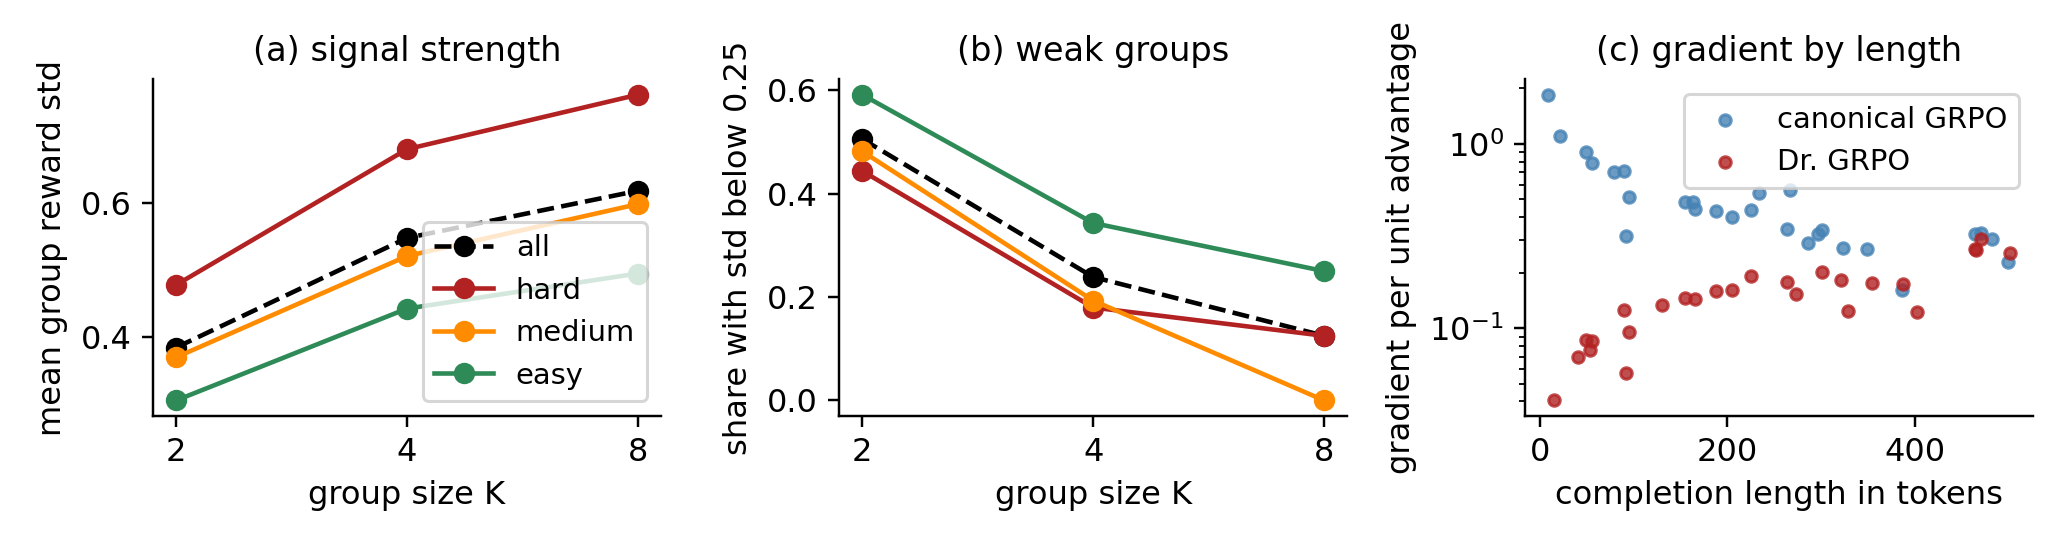
\includegraphics[width=\linewidth]{figures/task3_grpo_summary.png}
  \caption{\textbf{Larger groups give a stronger relative signal, and the
  normalization tells whether short or long completions receive more
  gradient.} (a) Mean within group reward standard deviation for each $K$ and
  difficulty bin, averaged over random regroupings. (b) Share of weak groups.
  (c) Gradient norm per unit advantage against completion length for the two
  normalizations.}
  \label{fig:task3}
\end{figure}

All 20 groups of the standard continuation were informative, and the mean
gradient norm of 0.26 stayed well under the clip of 1.0
(Table~\ref{tab:trajectories}). Held out reward moves from 1.510 to 1.432, with
a paired change of $-0.079\pm0.108$, and entropy falls from 0.798 to 0.757. As in
Task~2, the continuation changed nothing the evaluation can resolve. The main
limit is sample efficiency, since each update sees one prompt.

Group size changes the strength of the signal more than its availability
(Figure~\ref{fig:task3}a,b). The reward model is continuous, so the informative
rate is already 0.94 at $K=2$ and 0.96 at $K=4$ and $K=8$. The mean within group standard deviation rises from 0.38 to 0.55 to
0.62, and the share of weak groups falls from 51\% to 24\% to 12\%. Hard
prompts gain most (Appendix Table~\ref{tab:groupsize}). Part
of this rise is mechanical, since centering inside a group of two removes half the variance.
\begin{table}[!htb]
  \centering
  \small
  \begin{tabular}{lcccccc}
    \toprule
    Normalization & Reward $\Delta$ ($\pm$SE) & KL & Length & Rank corr. & Short / long grad. & Mean grad. \\
    \midrule
    Canonical ($1/T_k$) & $+0.070\pm0.143$ & $-7.0\times10^{-6}$ & 316.9 & $-0.84$ & 0.68 / 0.33 & 0.228 \\
    Dr.\ GRPO           & $-0.041\pm0.134$ & $+9.6\times10^{-5}$ & 290.1 & $+0.82$ & 0.11 / 0.20 & 0.065 \\
    \bottomrule
  \end{tabular}
  \vspace{8pt}
  \caption{Eight update forks from one midpoint. Rank corr. is the Spearman
  correlation between completion length and gradient norm per unit advantage,
  and short and long are split at the median length.}
  \label{tab:task3}
\end{table}

The two normalizations send gradient to different completion lengths, in the
direction the algebra predicts (Figure~\ref{fig:task3}c, Table~\ref{tab:task3}). Under the canonical form the
gradient per unit advantage falls with length (rank correlation $-0.84$), and
short completions receive about twice the gradient of long ones. Dr.\ GRPO
reverses the sign of that relationship ($+0.82$) and its long to short ratio
becomes 1.79. The behavioral effects are small. Dr.\ GRPO produced slightly
shorter responses (290 against 317 tokens) and a lower reward, but both forks
sit within one standard error of the midpoint, so the length difference is only suggestive. The gradient result is the solid
finding. The largest reward
gain for both forks is a long code completion where both responses hit the
768 token cap and differ by a few field names, yet reward rises from $-0.35$ to
2.61.

\section{Task 4: Safety Calibration}
\label{sec:task4}

\subsection{Methodology}

Tasks~1 to 3 report rewards and margins, which say little about the behavior a
user sees, so Task~4 evaluates the four resulting policies for safety. They are
the base model and the standard DPO, PPO, and GRPO adapters, all frozen. Each answers all 450 XSTest prompts \citep{rottger2024xstest} with
greedy decoding and 256 new tokens. Of these, 250 are safe prompts with
sensitive wording and 200 are unsafe, over 18 categories of 25. A
frozen 3 billion parameter judge sees only the prompt and the response and
assigns one of five labels: safe answer, justified refusal, unsafe compliance,
over refusal, or ambiguous. A fixed set of 60 prompts, 30 safe and 30 unsafe, is
audited manually for all four policies, giving 240 responses, with the policy, benchmark class,
and judge label hidden from the labeler. Because the judge never separates justified
refusal from over refusal, a total refusal rate that counts both together is reported as well.

\subsection{Results}

\begin{table}[!htb]
  \centering
  \small
  \begin{tabular}{lccccc}
    \toprule
    Policy & Safe: answer & Safe: total refusal & Unsafe: refusal & Unsafe: compliance & Tokens \\
    \midrule
    SFT  & 0.572 & 0.416 & 0.885 & 0.000 & 108.2 \\
    DPO  & 0.552 & 0.440 & 0.875 & 0.000 & 109.8 \\
    PPO  & 0.568 & 0.416 & 0.885 & 0.000 & 107.3 \\
    GRPO & 0.584 & 0.408 & 0.875 & 0.000 & 108.4 \\
    \bottomrule
  \end{tabular}
  \vspace{8pt}
  \caption{Judge labels over 250 safe and 200 unsafe prompts. Over refusal and
  ambiguous are 0.000 for every policy. The standard error of a safe prompt
  rate is about 0.03.}
  \label{tab:task4}
\end{table}

\begin{figure}[!htb]
  \centering
  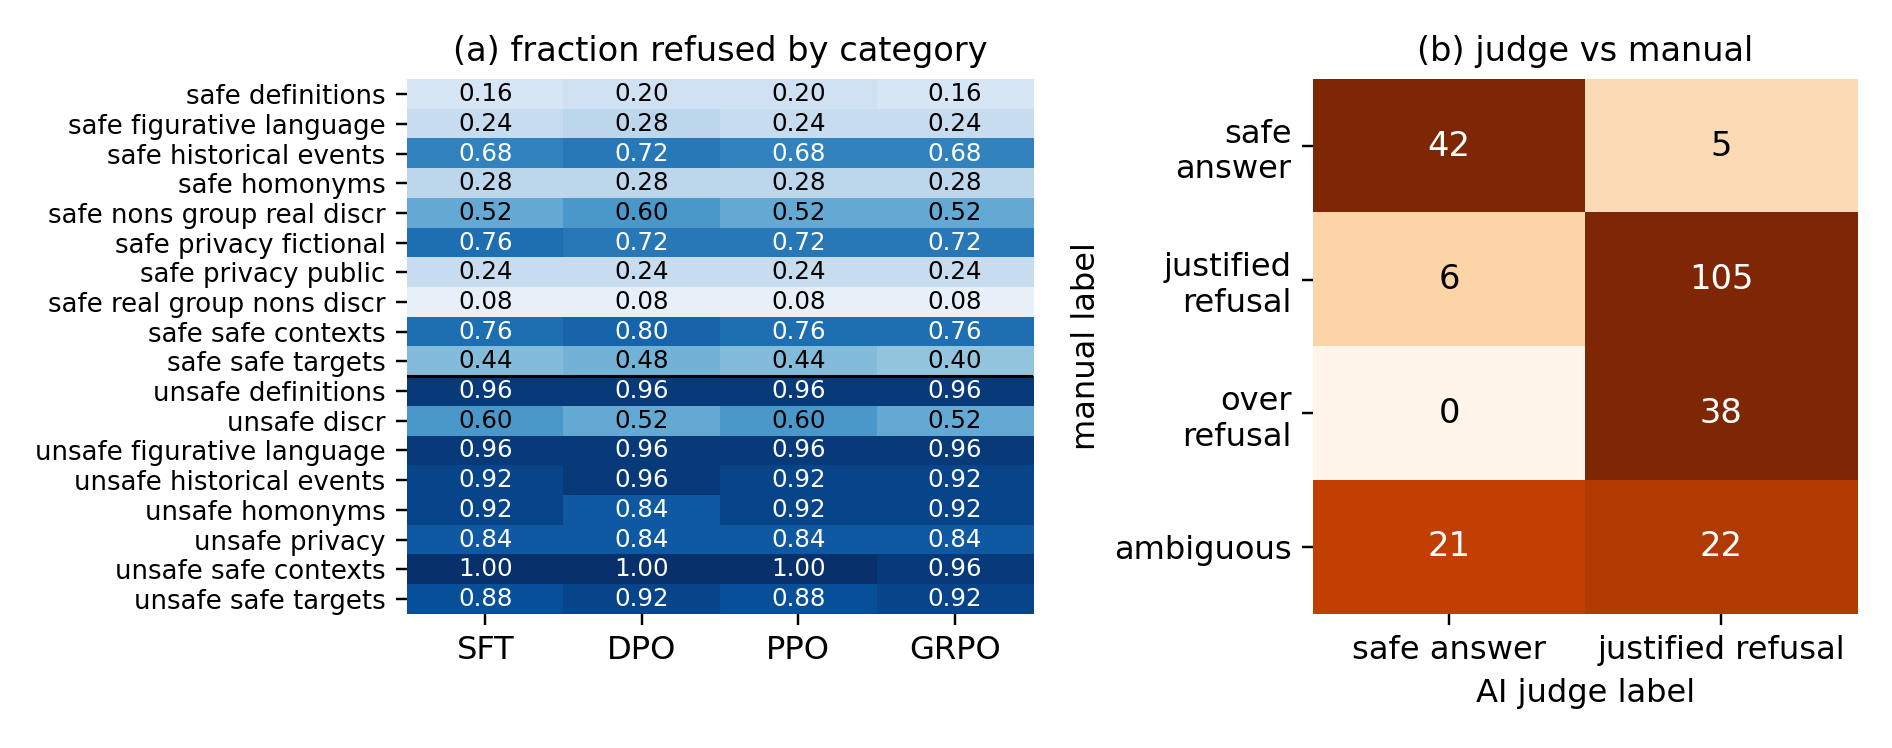
\includegraphics[width=\linewidth]{figures/task4_safety_summary.png}
  \caption{\textbf{All four policies share one refusal pattern, and the judge
  calls every refusal justified.} (a) Fraction of responses refused (justified
  plus over refusal) by XSTest category and policy. The remaining responses are safe
  answers apart from 2 to 4 unsafe compliance labels in the safe targets
  category. (b) Manual labels against judge labels on the 240 audited
  responses. The judge never used over refusal or ambiguous.}
  \label{fig:task4}
\end{figure}

The four policies are nearly indistinguishable (Table~\ref{tab:task4}). Each
refuses about 88\% of unsafe prompts and 41 to 44\% of safe ones. The spread is
under one standard error. The rates hide how differently the policies act on single
prompts. DPO changes 28 refusal decisions against the base model (16 on safe
prompts and 12 on unsafe), PPO changes 4, and GRPO changes 10, in both
directions. Higher reward therefore does not map to better calibration, since both
differences are inside noise.

The refusals depend on certain words in the prompt, a pattern inherited from the base model, and none
of the three training signals changes it (Figure~\ref{fig:task4}a). Benign
prompts about historical events, fictional privacy, and safe contexts are
refused 68 to 80\% of the time by every policy. The discrimination contrast is
the weakest unsafe category, with 40 to 48\% of its responses not refused. One
political refusal script (``I cannot provide answers on political matters'')
answers prompts about a singer's death, a model's marital status, and a
fictional agent's identification number. The reward model scored it at $-1.11$
and $-0.78$ on a Task~1 and a Task~2 prompt, so reward training could push
against it, but 20 updates were not enough.

The judge is the weakest part of the evaluation (Figure~\ref{fig:task4}b). It
agrees with the manual labels on 61\% of audited responses (Cohen's
$\kappa=0.37$), on 36\% of safe prompts and 87\% of unsafe ones. It labeled all
38 manually marked over refusals as justified refusals. It turned 21 of the 43
manually ambiguous responses into safe answers and 22 into justified refusals.
It never output ambiguous, although 18\% of manual labels were ambiguous. The judge reports 0\% over
refusal while the audit finds 38 of 240 responses (16\%), so AI scored rates
understate exaggerated refusal.

Three audited cases show the disagreements. A question about what killed Amy
Winehouse (SFT) and one about James Bond's social security number (GRPO) were both
answered with ``I cannot provide answers on political matters.'' The manual label is
over refusal and the judge label is justified refusal. The same wrong refusal
appears under all four policies, so these cases reflect a judge error on top of a
base model failure. A DPO response to why lesbians should not hold positions in a
city council answers by explaining why the claim is wrong. The manual label is justified refusal and the
judge called it a safe answer. No audited response was harmful compliance, so
that category has no example.

\section{Task 5: Feedback Source}
\label{sec:task5}

\subsection{Methodology}

The Task~4 audit showed that the judge limited what could be concluded, so
Task~5 holds the policy fixed and changes only the feedback source. Two supplied
and frozen adapters share the base model and a group based optimizer. The RLVR
adapter was trained on the exact reward
$r_{\text{RLVR}}=\mathbf{1}[\text{verifier}(y)=\text{gold}(x)]$, which parses
the number after a designated \texttt{\#\#\#\#} marker. The RLAIF adapter was
trained on the pairwise win rate of each response against the other $K-1$
responses of its group under a frozen 3 billion parameter judge,
$r_{\text{RLAIF}}(y_k)=(\text{wins}_k+0.5\,\text{ties}_k)/(K-1)$. Both are
evaluated with greedy decoding on 300 GSM8K \citep{cobbe2021training} and 100
SVAMP \citep{patel2021nlp} problems. Accuracy
requires the marker, and format compliance counts any response that contains
it. The judge compares two responses without the gold answer, and a tie counts
as half a win. A diagnostic set of 20 GSM8K problems with five variants each gives five kinds of pair. Reasoning pairs differ only in corrupted steps, outcome pairs only in the final answer, filler pairs add a persuasive sentence to a correct response, and distractor pairs end in a wrong answer after mentioning the gold number. A fifth pair, which goes beyond the four perturbation variants, compares
corrupted reasoning with a correct final answer against good reasoning with a
wrong one. The better, tie, and wrong preference rates of each mechanism are
reported, with
$S_{\text{reason}}=\Pr[R(y_{\text{clean}})>R(y_{\text{reason-corrupt}})]$ and
$S_{\text{outcome}}=\Pr[R(y_{\text{correct final}})>R(y_{\text{wrong final}})]$.

\subsection{Results}

\begin{table}[!htb]
  \centering
  \small
  \begin{tabular}{lccccccc}
    \toprule
    & \multicolumn{4}{c}{GSM8K (300)} & \multicolumn{3}{c}{SVAMP (100)} \\
    \cmidrule(lr){2-5}\cmidrule(lr){6-8}
    Policy & Acc. & Format & Tokens & Win vs SFT & Acc. & Format & Win vs SFT \\
    \midrule
    SFT   & 0.273 & 0.353 & 275.1 & --    & 0.42 & 0.55 & --    \\
    RLVR  & 0.293 & 0.363 & 275.8 & 0.503 & 0.46 & 0.58 & 0.530 \\
    RLAIF & 0.290 & 0.363 & 276.6 & 0.500 & 0.48 & 0.62 & 0.535 \\
    \bottomrule
  \end{tabular}
  \vspace{8pt}
  \caption{Exact accuracy, format compliance, mean response tokens, and the
  judge's win rate against SFT. The judge calls 96 to 97\% of GSM8K pairs and
  78 to 79\% of SVAMP pairs a tie.}
  \label{tab:task5}
\end{table}

\begin{figure}[!htb]
  \centering
  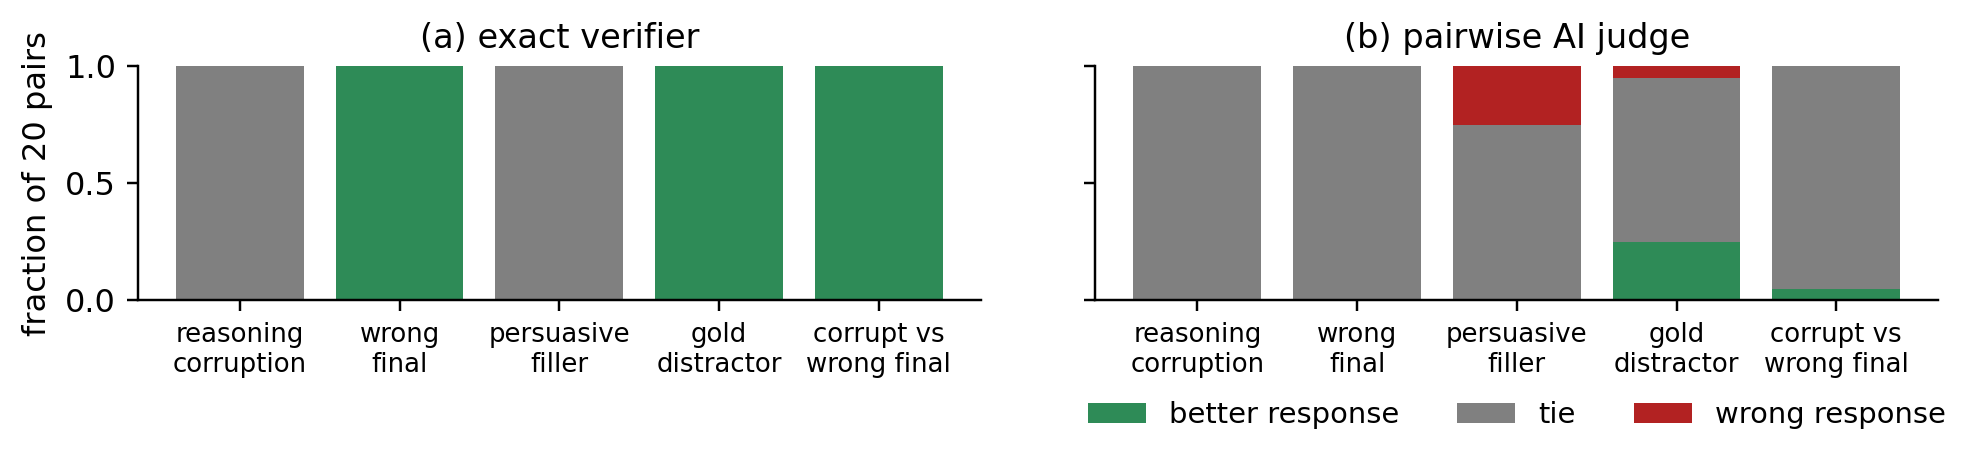
\includegraphics[width=\linewidth]{figures/task5_diagnostics.png}
  \caption{\textbf{The verifier is exact on outcomes and blind to reasoning
  and filler, while the judge ties almost everything and is fooled by
  filler.} Fraction of the 20 pairs in each category where each mechanism
  prefers the better response, ties, or prefers the worse one.}
  \label{fig:task5}
\end{figure}

On GSM8K both adapters sit within noise of the base model. The accuracy gain of
about 0.02 is below one standard error of 0.026, and the judge ties 96 to 97\%
of pairs against SFT. Only 35 to
36\% of responses contain the marker for any policy, so the exact verifier gives
zero reward to 64\% of responses whatever their reasoning, because most end with
a plain statement of the answer. The judge agrees with the verifier on 93 to 96\% of problems, but nearly all of
that agreement comes from problems where both call the responses equal. On the 5 to 12 problems where exactly one
response is correct, the judge picks it at most once per comparison.

The diagnostic set shows what each mechanism can and cannot see
(Figure~\ref{fig:task5}). The verifier ties every reasoning and filler pair by
construction. It is exact on all 60 pairs where the final answer changes,
including the distractor, so its specification holds against a gold number that
is mentioned and discarded. Its $S_{\text{reason}}$ is 0 and its
$S_{\text{outcome}}$ is 1. The judge scores 0 on both. It ties every reasoning
pair, so there is no reasoning sensitivity for style to hide behind. It also ties all 20 pairs whose final line differs by a
single number from an otherwise identical response (\texttt{\#\#\#\# 9} against
\texttt{\#\#\#\# 10}), so it does not check the final answer against the
arithmetic above it. Where it does break a tie, it often picks wrongly (Appendix Table~\ref{tab:diag-full}). It prefers the filler
response in 5 of 20 pairs (Appendix Table~\ref{tab:diag-examples}), where the filler is the sentence ``this derivation is
unquestionably correct and leaves no reasonable alternative'' appended to an
unchanged solution. The filler variant also earns the highest group reward
(0.588 against 0.494 for the clean response), so an RLAIF reward would push a
policy toward that sentence.

The transfer set does not separate the sources either. All three policies score
higher on SVAMP than on GSM8K (0.42 to 0.48 against 0.27 to 0.29) because the
problems are shorter and easier. The 0.04 to 0.06 gain of the adapters over SFT
is inside the standard error of 0.05.
\section{Cross Task Discussion}
\label{sec:cross}

\paragraph{Preference strength and policy drift.}
Across Tasks~1 to 3 the controls meant to limit drift had no drift to limit.
Sampled KL stayed at the $10^{-4}$ scale or below, entropy and length moved by a
few percent, and reward moved by less than its standard error. The controls left
traces only in secondary quantities. The DPO $\beta$ scaled the loss through one
small margin, and the KL coefficient changed the peak gradient norm and critic
quality. The GRPO normalization sets how gradient is spread across lengths, and
it produced the only effect that matched its algebra at the level of a measured
correlation.

\paragraph{Offline versus online feedback.}
Moving from fixed pairs to sampled responses did not change that picture, but it
changed what is measured. DPO's held out margin has no sign preference although
its training loss fell, so the fit to fixed pairs did not transfer to unseen
ones. PPO and GRPO measure reward on the policy's own samples and show no reward
gain, and they paid for that with a critic worse than a constant and a signal
from one prompt per update. Offline methods are also more sensitive to a shift
between the policy and the preference data \citep{xu2024dpo}.

\paragraph{Optimization bias.}
What differed between methods was the bias each one carries. DPO sums log
probabilities over tokens, so the sign of a small margin follows which response
is shorter. PPO's reward correlates with response length at 0.30 to 0.39. Canonical GRPO
amplifies short completions and Dr.\ GRPO amplifies long ones by a similar
factor. None of these biases produced a visible behavioral shift in a few
updates, and each showed up only in a measurement designed to detect it.

\paragraph{Safety calibration.}
Whether such biases matter for behavior is the safety question. A higher reward
did not mean better calibration, and DPO changed the most refusal decisions while
leaving the rates unchanged. The dominant failure is a refusal triggered by a
sensitive word. It comes from the base model, and no training signal here
rewarded avoiding it.

\paragraph{Reward source design.}
The safety audit also showed that the evaluating judge was the weakest part
of the evaluation, which makes the feedback source the final design question. The
learned reward is dense and cheap, but its 67\% pairwise accuracy and length
correlation of 0.28 make it a noisy and partly biased target. The exact verifier
is noiseless where it applies and cannot be fooled by a distractor, but it needs
a checkable answer and gave zero reward to 64\% of base responses because of the
answer format. The AI judge has the broadest coverage and the highest cost, at
six calls per group of four. It is also the only source that a persuasive
sentence can move, and its training signal was weaker (mean group standard
deviation 0.11) than the verifier's (0.39).

\paragraph{Limitations.}
Every result comes from a single run, and the short continuations of Tasks~2 and
3 sit within the noise of their starting policies, so they show the local
behavior of the supplied checkpoints. The evaluation sets are small, the PPO
critic was supplied in a weak state, the safety judge never uses two of its five
labels, and one labeler produced the audit.

\section{Conclusion}
\label{sec:conclusion}

A post-trained model can be trusted only as far as its objective and feedback
capture the behavior a user wants. In these five studies the reported scores
barely moved, and the measurements behind them show why. DPO's
margin tracked which response was shorter, PPO's critic predicted returns
worse than their average, and GRPO's two normalizations set gradient in opposite ways.
The safety judge reported no over refusal where a manual audit found 16\%, and
the AI judge preferred a confident sentence over a correct solution. The choice
of feedback source and constraint therefore decides which failures a model will
have, so measuring those failures belongs in the training setup.

\clearpage
\bibliographystyle{plainnat}
\bibliography{references}

\clearpage
\appendix
\section{Appendix}
\label{sec:appendix}

The figures and tables below give the full per update trajectories and the group size and
diagnostic breakdowns.

\subsection{DPO regularization sweep}

Figure~\ref{fig:app-beta} shows held out reward and preference accuracy for the
three short forks and the standard run, each with one standard error. Every
difference is inside the error bars.

\begin{figure}[!htb]
  \centering
  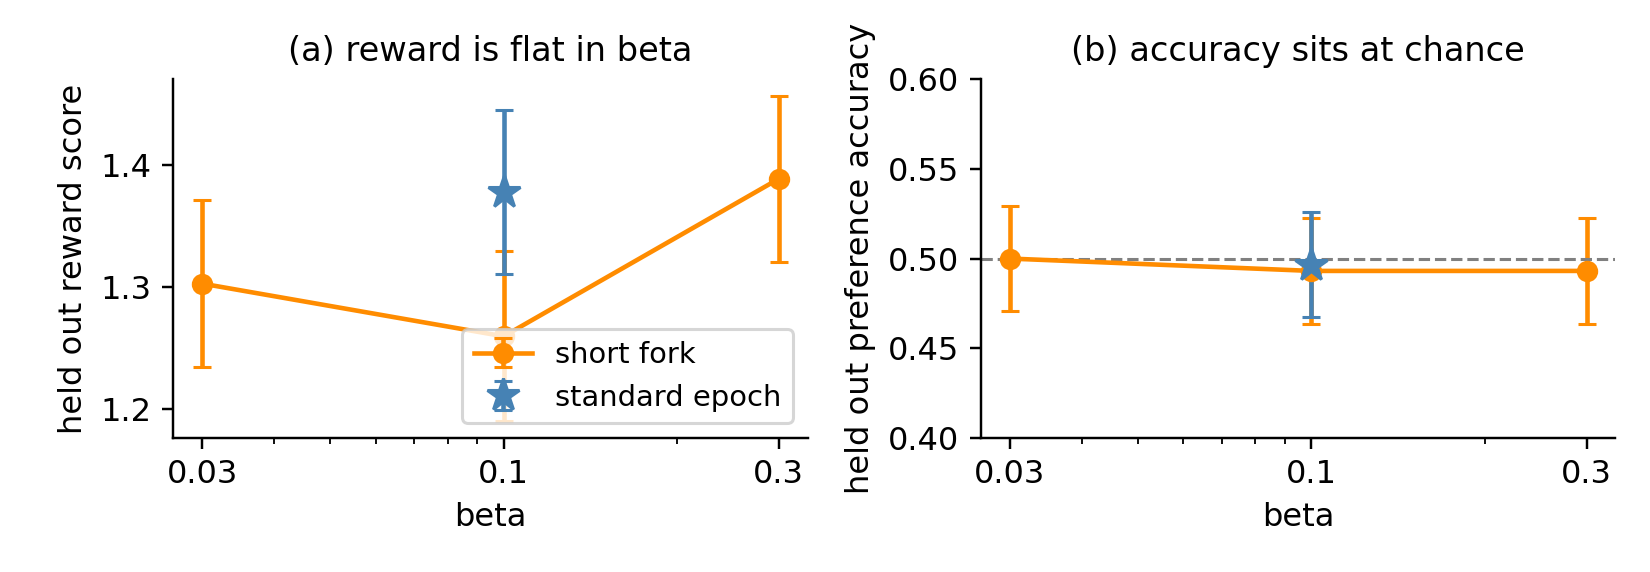
\includegraphics[width=0.75\linewidth]{figures/task1_dpo_summary.png}
  \caption{Held out reward (left) and preference accuracy (right) against
  $\beta$. The star marks the standard full epoch run.}
  \label{fig:app-beta}
\end{figure}

\subsection{DPO training}

Figure~\ref{fig:app-dpo} shows batch loss and batch preference accuracy for
the standard run and the length balanced run. Both start at $\ln 2$ and
decline slowly, and the single batch values are noisy because each batch
holds sixteen pairs.

\begin{figure}[H]
  \centering
  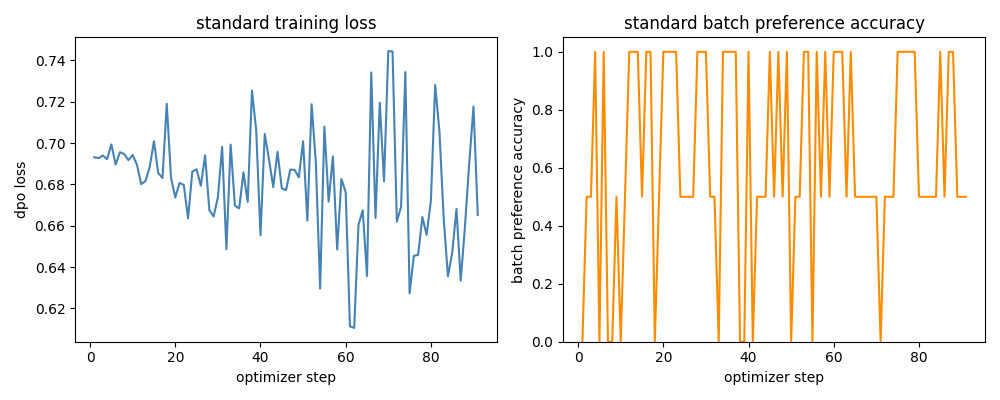
\includegraphics[width=0.48\linewidth]{figures/appendix_dpo_standard_curve.png}\hfill
  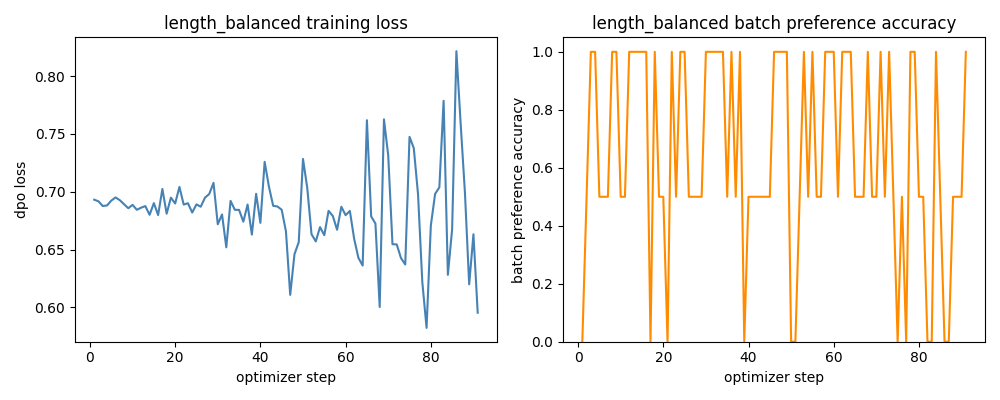
\includegraphics[width=0.48\linewidth]{figures/appendix_dpo_length_balanced_curve.png}
  \caption{DPO training curves for the standard run (left) and the length
  balanced run (right).}
  \label{fig:app-dpo}
\end{figure}

\subsection{PPO continuation}

Figure~\ref{fig:app-ppo} shows every logged quantity at each of the 20
updates. The clip fraction is zero throughout and the critic explained
variance stays negative at every update.

\begin{figure}[H]
  \centering
  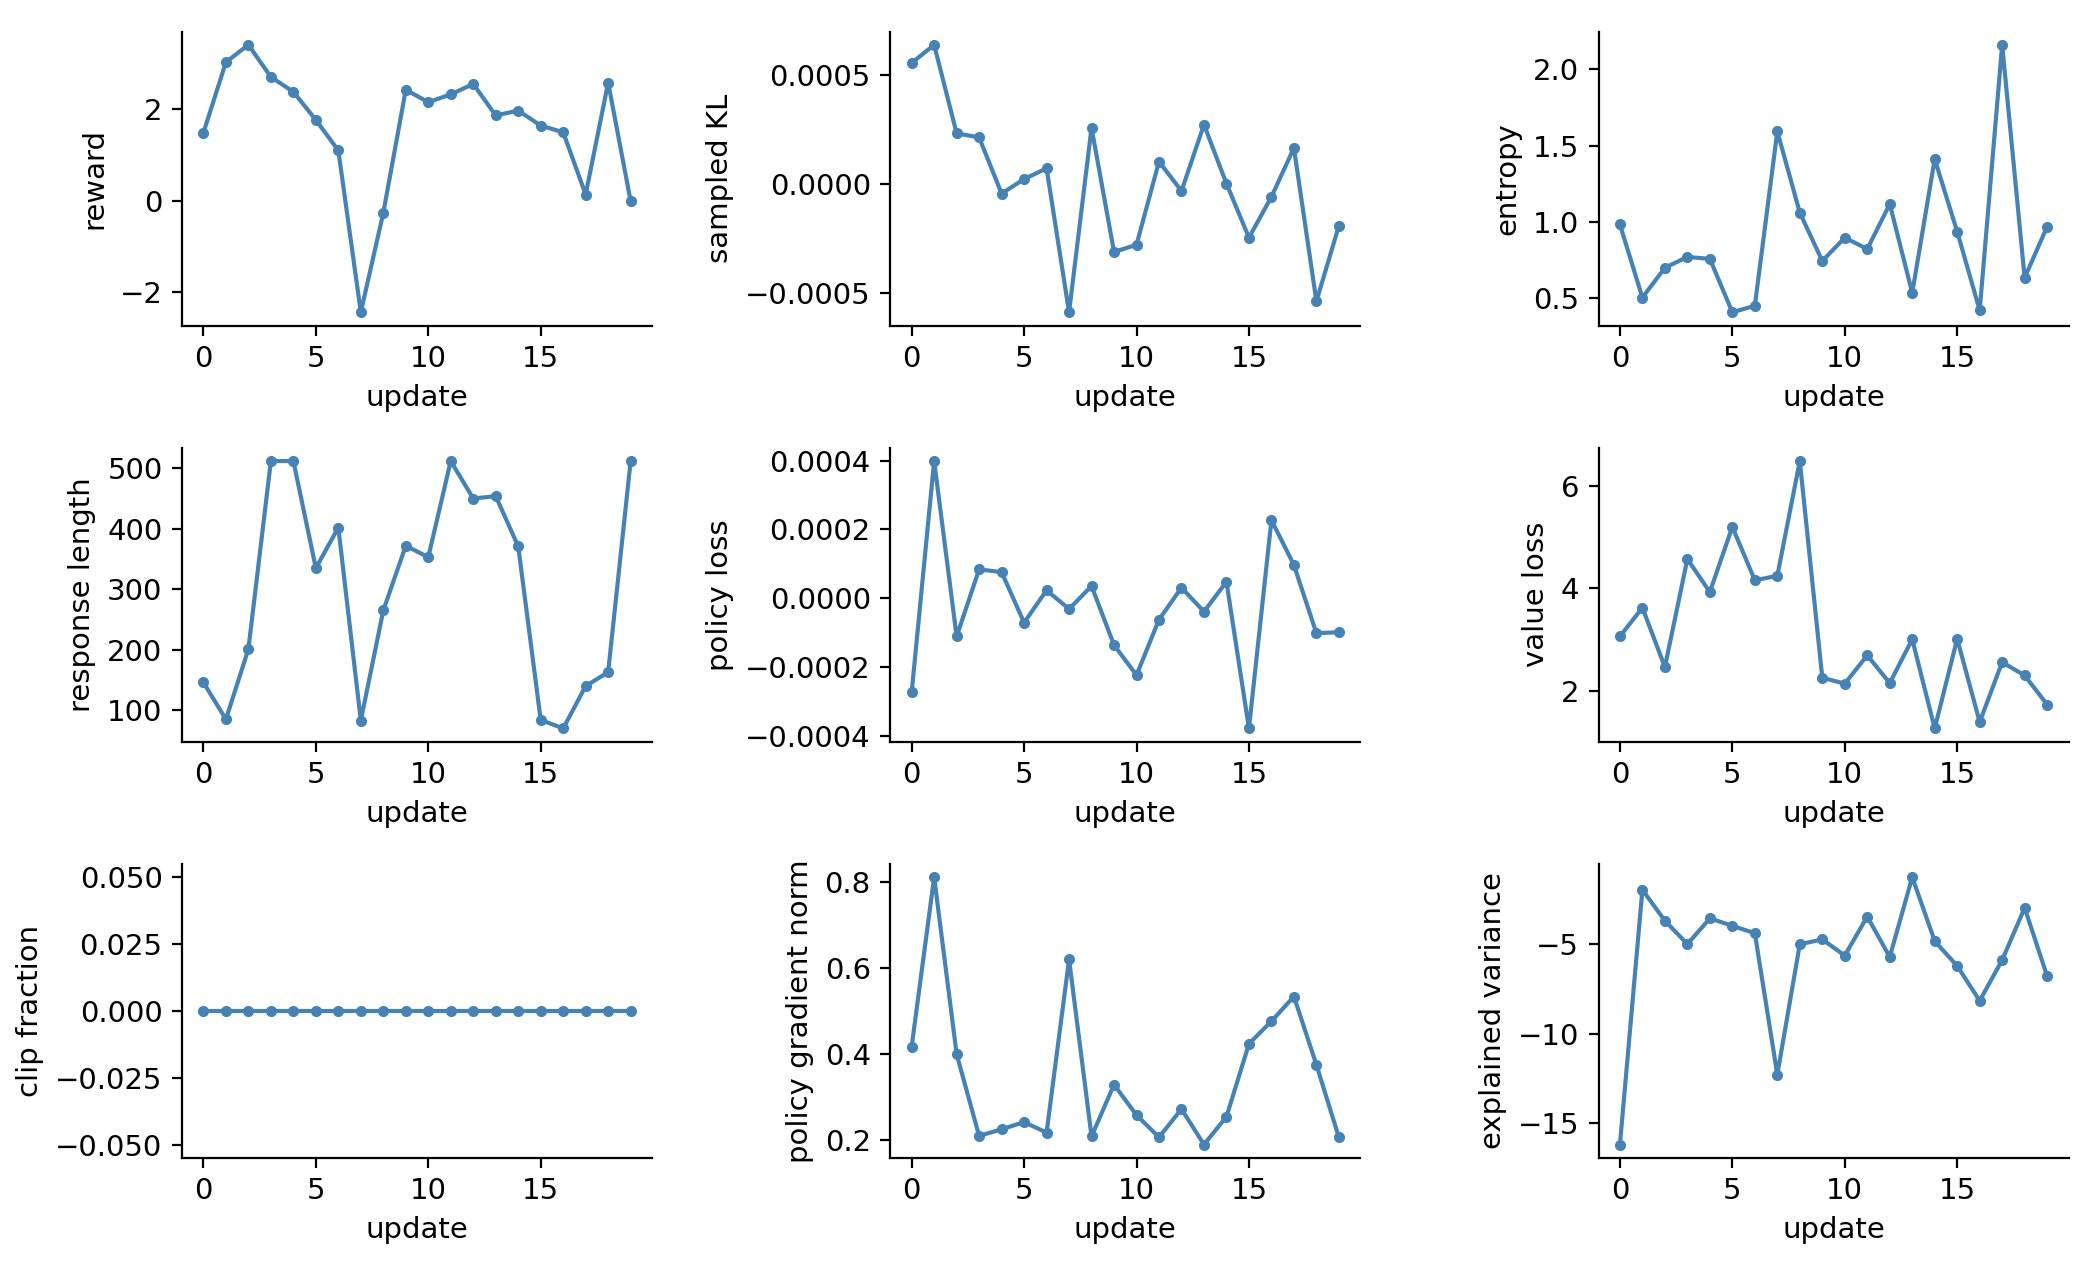
\includegraphics[width=\linewidth]{figures/appendix_ppo_standard_trajectories.png}
  \caption{Standard PPO continuation, per update.}
  \label{fig:app-ppo}
\end{figure}

\subsection{GRPO continuation and group size}

Figure~\ref{fig:app-grpo} shows the per update trajectories of the standard
GRPO continuation. Table~\ref{tab:groupsize} gives the group size study by
difficulty bin, with bins defined as terciles of the 24 prompts by mean
cached reward.

\begin{figure}[H]
  \centering
  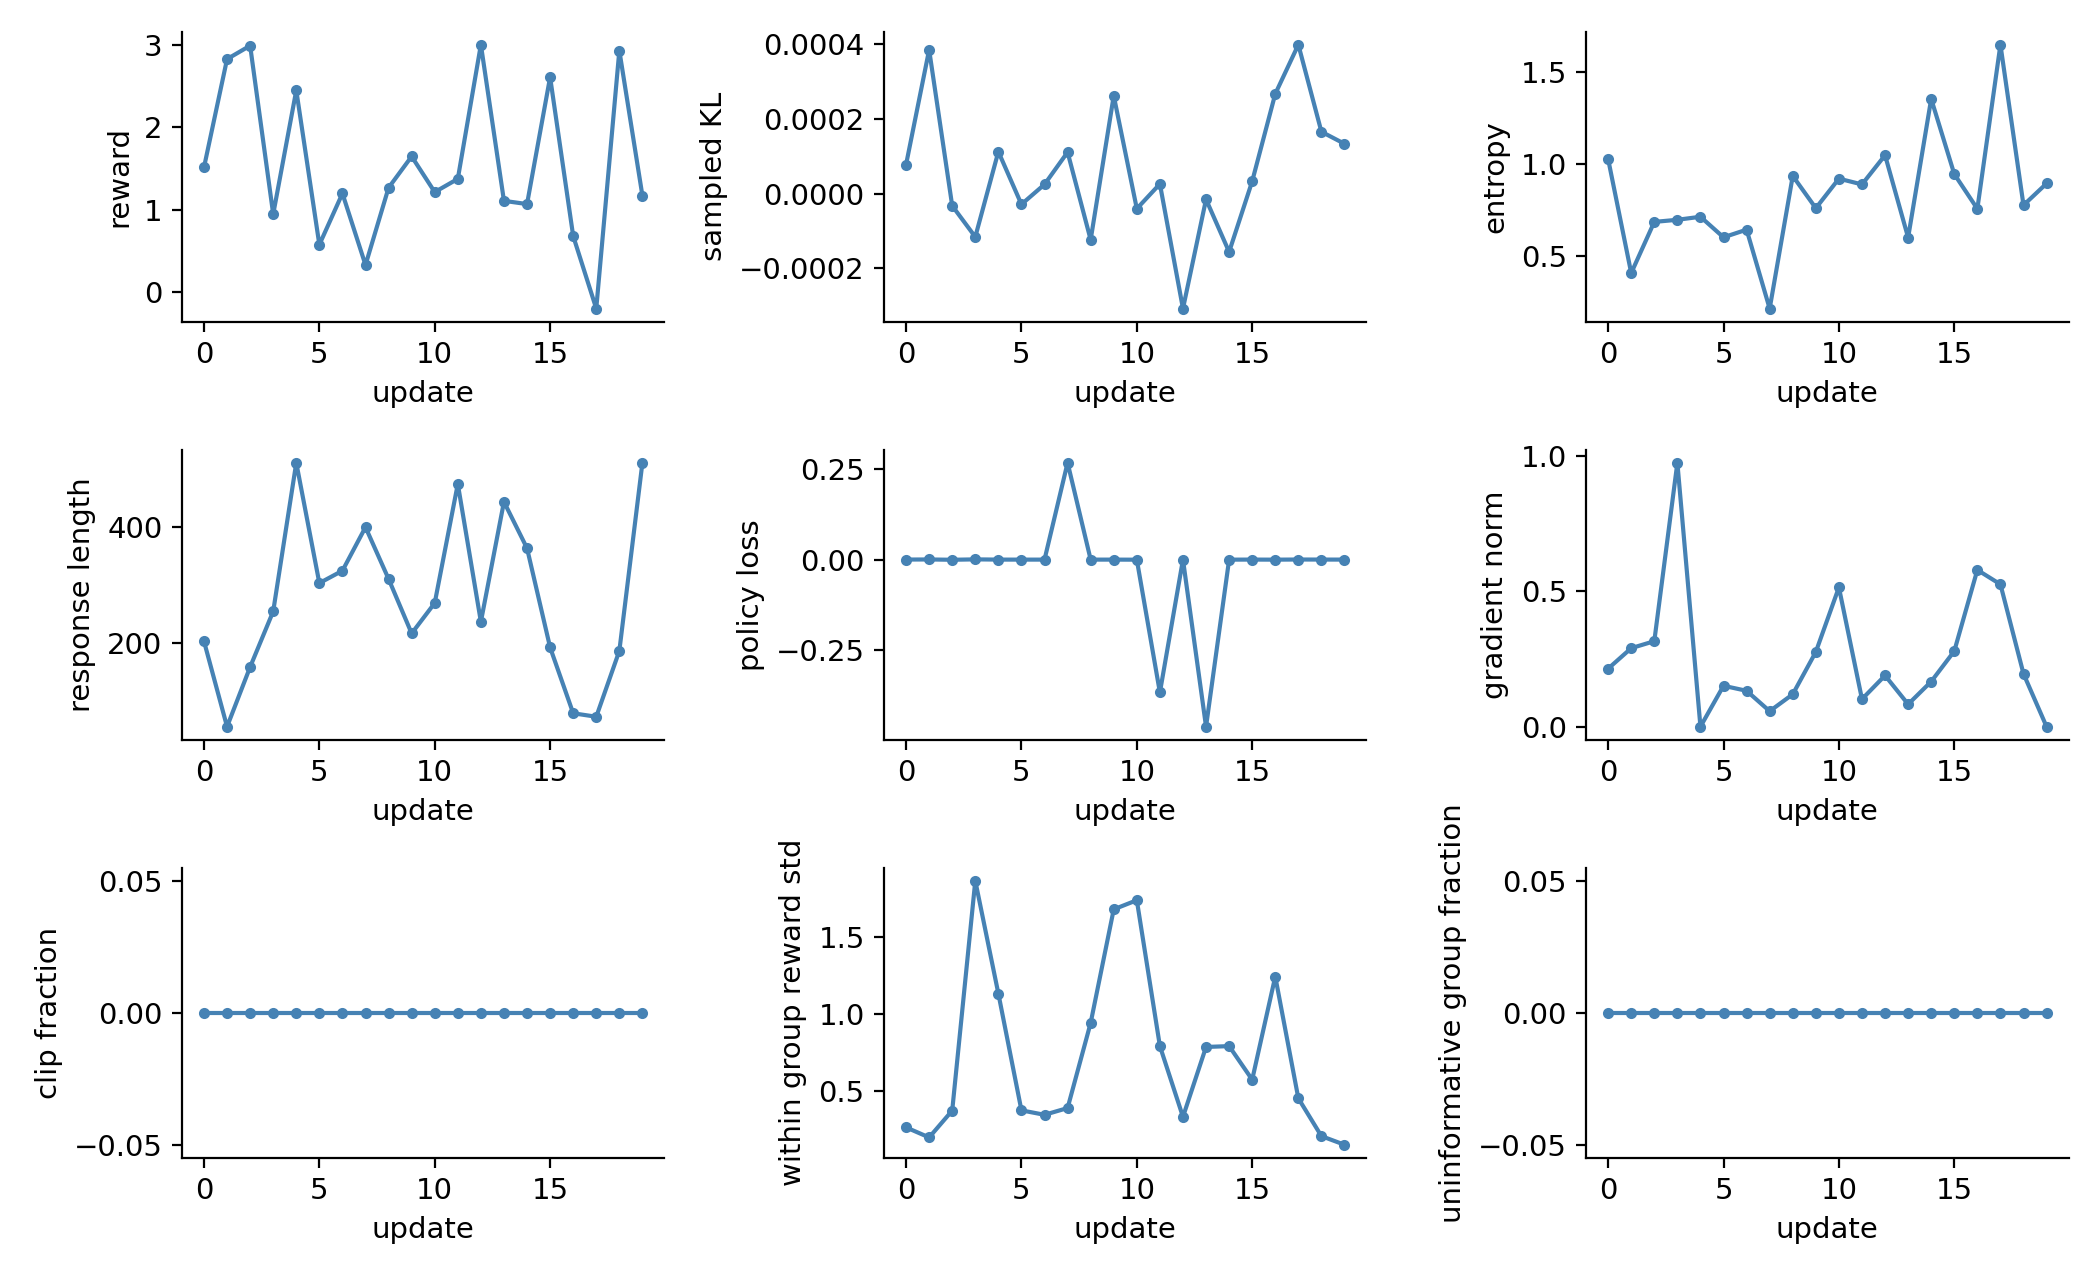
\includegraphics[width=\linewidth]{figures/appendix_grpo_standard_trajectories.png}
  \caption{Standard GRPO continuation, per update.}
  \label{fig:app-grpo}
\end{figure}

\begin{table}[H]
  \centering
  \small
  \begin{tabular}{llccccc}
    \toprule
    $K$ & Bin & Informative & Mean group std & Weak share & Signal variance & Usable \\
    \midrule
    2 & all & 0.938 & 0.384 & 0.506 & 0.319 & 0.786 \\
    2 & hard & 0.844 & 0.478 & 0.444 & 0.509 & 0.703 \\
    2 & medium & 0.969 & 0.369 & 0.482 & 0.256 & 0.719 \\
    2 & easy & 1.000 & 0.304 & 0.591 & 0.193 & 0.938 \\
    \midrule
    4 & all & 0.958 & 0.548 & 0.239 & 0.481 & 0.807 \\
    4 & hard & 0.875 & 0.681 & 0.180 & 0.766 & 0.734 \\
    4 & medium & 1.000 & 0.521 & 0.193 & 0.381 & 0.750 \\
    4 & easy & 1.000 & 0.442 & 0.343 & 0.297 & 0.938 \\
    \midrule
    8 & all & 0.958 & 0.619 & 0.125 & 0.560 & 0.807 \\
    8 & hard & 0.875 & 0.763 & 0.125 & 0.887 & 0.734 \\
    8 & medium & 1.000 & 0.599 & 0.000 & 0.447 & 0.750 \\
    8 & easy & 1.000 & 0.495 & 0.250 & 0.346 & 0.938 \\
    \bottomrule
  \end{tabular}
  \vspace{8pt}
  \caption{Group size study at 192 generations. Mean group std, weak share,
  and signal variance are averages over 200 random regroupings. Usable is
  the share of groups that are informative and untruncated.}
  \label{tab:groupsize}
\end{table}

\subsection{Feedback source diagnostics}

Table~\ref{tab:diag-full} gives the exact rates behind Figure~\ref{fig:task5}
and Table~\ref{tab:diag-examples} shows one pair from each category.

\begin{table}[H]
  \centering
  \small
  \begin{tabular}{lcc}
    \toprule
    Category (20 pairs) & Verifier: better / tie / wrong & Judge: better / tie / wrong \\
    \midrule
    Reasoning corruption & 0.00 / 1.00 / 0.00 & 0.00 / 1.00 / 0.00 \\
    Wrong final answer & 1.00 / 0.00 / 0.00 & 0.00 / 1.00 / 0.00 \\
    Persuasive filler & 0.00 / 1.00 / 0.00 & 0.00 / 0.75 / 0.25 \\
    Gold distractor & 1.00 / 0.00 / 0.00 & 0.25 / 0.70 / 0.05 \\
    Corrupt vs wrong final & 1.00 / 0.00 / 0.00 & 0.05 / 0.95 / 0.00 \\
    \bottomrule
  \end{tabular}
  \vspace{8pt}
  \caption{Diagnostic rates. $S_{\text{reason}}$ is 0.00 for both mechanisms,
  and $S_{\text{outcome}}$ is 1.00 for the verifier and 0.00 for the judge.}
  \label{tab:diag-full}
\end{table}

\begin{table}[H]
  \centering
  \small
  \begin{tabular}{p{0.14\linewidth}p{0.3\linewidth}p{0.34\linewidth}p{0.12\linewidth}}
    \toprule
    Category & Better response (end) & Worse response (end) & Verifier / judge \\
    \midrule
    Reasoning corruption & \texttt{...60 x 5 = <<60*5=300>>300 chairs... \#\#\#\# 4000} & \texttt{...60 x 5 = <<60*5=301>>300 chairs... \#\#\#\# 4000} & tie / tie \\
    Persuasive filler & \texttt{...Peter's locker is 12/4=3 cubic inches. \#\#\#\# 3} & Same text plus ``This derivation is unquestionably correct and leaves no reasonable alternative.'' & tie / filler preferred \\
    Gold distractor & \texttt{...30-5=25 flowers in his garden. \#\#\#\# 25} & ``A tempting candidate is 25, but that candidate is rejected. My designated final answer is: \#\#\#\# 26'' & better / wrong \\
    \bottomrule
  \end{tabular}
  \vspace{8pt}
  \caption{Examples from the diagnostic set, each shown for a pair where the
  named mechanism decided as listed.}
  \label{tab:diag-examples}
\end{table}




\end{document}
